\section{Problem Statement}
In order to develop bathymetric prediction models we must first decide what types of inputs will be used to calculate results. 
For the scope of this project the choice was made to compute statistically derived values from existing bathymetry data sets. 
Bathymetry data is gridded data where a single grid value represents the elevation of a physical location on Earth. 
Imagine a grid where each row represents a latitude value and each column represents a longitude value. 
This would produce a grid with 64,800 entries (360 x 180). 
Now if we have to compute a statistical value for each grid cell we would need to perform 64,800 computations. 
Since statistical computations such as mean and standard deviation require evaluating a series of data values, we have to look at each grid cells’ neighbors out to some point. 
Therefore, in this example, we have to process 64,800 “mini” grids to get the desired results. 
To complicate things further, a one degree by one degree cell represents several square miles of Earth. 
Assigning a single elevation value to such a large space is not practical in that it does not give a true representation of the physical makeup of the Earth. 
For a more accurate depiction, higher resolution data sets are needed. 
The drawback is the more accurate the depiction, the larger the data set required to store the information. 
The table below shows existing bathymetry products currently available and the amount of grid cells needed to represent the elevation data.

\begin{figure}[h]
    \centering
    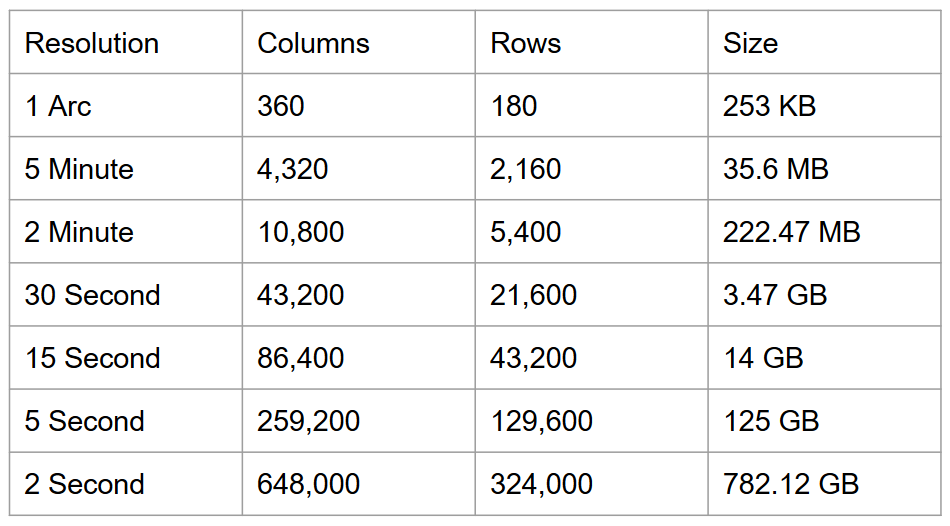
\includegraphics[scale=0.5]{grid_sizes}
    \caption{Graphic showing the sizes of grid files}
    \label{fig2:Figure 2}
\end{figure}

\par
Based on the information in Figure 2 you can see how the number of computations required to produce statistical and mathematically derived data can grow as the resolution of the underlying bathymetry product gets higher.
In addition to the data size issue, the types of inputs needed to obtain optimal results is an unknown. 
Based on prior work, the geophysicists will make assumptions and estimates on which types of input values could potentially produce acceptable results. 
These assumptions will be used to generate a series of input values used in model training and evaluation. 
If acceptable results are not produced, new assumptions are made and additional datasets will need to be created. 
This iterative process could occur several times over the course of this study; therefore, it is imperative for the input data generation process to be as efficient as possible.

\par
The purpose of our class project is to design a series of programs that will use varying types of parallelization to compute statistical and mathematically derived data sets for use in bathymetric prediction model training. 
These data sets will be computed from large high resolution existing bathymetry data sets based on guidance from the geophysicists working this effort. 
The goal is to find the most optimal implementations for performing grid based computation to produce enough prediction model input to test a breadth of input types to obtain meaningful results.
